\documentclass[review, onefignum, onetabnum]{siamart171218}
% This is information that is shared between the main document and any
% supplement. If no supplement is required, then this information can
% be included directly in the main document.


% Packages and macros go here
\usepackage{lipsum}
\usepackage{amsfonts}
\usepackage{graphicx}
\usepackage{epstopdf}
\usepackage{algorithmic}
\usepackage{tikz}
\usepackage{subcaption} 
\usepackage{pc_math}
\usepackage{amssymb}
\usepackage{bbm}
% \usepackage[color=gray!60]{todonotes}
\usepackage[disable, color=gray!60]{todonotes}
% \usepackage{caption}
% \usepackage{hyperref}
\graphicspath{{fig/}}

\tikzstyle{major}=[circle, fill=blue!50, minimum size=10pt, line width=0mm, inner sep=0pt, draw=black]
\tikzstyle{minor} = [major, fill=orange!80, draw=black]
\tikzstyle{focus} = [minor, line width=.2mm, inner sep=1pt, draw=black]
\tikzstyle{edge} = [draw,line width=.3mm, -, gray!120]
\tikzstyle{gone} = [edge,  densely dotted]
\tikzstyle{arrow} = [draw,line width=.2mm, ->, gray!120]


\tikzstyle{weight} = [font=\small]

\ifpdf
  \DeclareGraphicsExtensions{.eps,.pdf,.png,.jpg}
\else
  \DeclareGraphicsExtensions{.eps}
\fi

% Add a serial/Oxford comma by default.
\newcommand{\creflastconjunction}{, and~}

% Used for creating new theorem and remark environments
\newsiamremark{remark}{Remark}
\newsiamremark{hypothesis}{Hypothesis}
\crefname{hypothesis}{Hypothesis}{Hypotheses}
\newsiamthm{claim}{Claim}

% Sets running headers as well as PDF title and authors
\headers{Adaptive Voter Models}{P. Chodrow, P. J. Mucha}

% Title. If the supplement option is on, then "Supplementary Material"
% is automatically inserted before the title.
\title{Local Symmetry-Breaking Drives Global Structure-Formation in Adaptive Networks\thanks{Submitted to the editors \today.
\funding{This work was funded by the NSF (1122374).}}}

% Authors: full names plus addresses.
\author{Philip S. Chodrow\thanks{Operations Research Center, Massachusetts Institute of Technology, Cambridge, MA, 02139 and Laboratory for Information and Decision Systems, Massachusetts Institute of Technology, Cambridge, MA, 02139
  (\email{pchodrow@mit.edu}, \url{http://www.philchodrow.github.io}).}
\and Peter J. Mucha\thanks{Carolina Center for Interdisciplinary Applied Mathematics, Department of Mathematics, University of North Carolina, Chapel Hill, NC 27599-3250, and Department of Applied Physical Sciences, University of North Carolina, Chapel Hill, NC 27599-3050. 
  (\url{http://mucha.web.unc.edu/}).}}

\usepackage{amsopn}
%%% Local Variables: 
%%% mode:latex
%%% TeX-master: "ex_article"
%%% End: 


\usepackage{cite}

\usepackage{color}
\usepackage{xcolor}
\colorlet{comment_purple}{blue!50!red}

\usepackage{todonotes}

\newcommand{\pjm}[1]{{\color{blue}[PJM: #1]}}
\newcommand{\pc}[1]{{\color{comment_purple}[PC: #1]}}
\ifpdf
  \hypersetup{
    pdftitle={Adaptive Voter Models},
    pdfauthor={P. Chodrow, P. J. Mucha}
  }
\fi

\begin{document}
\maketitle

\begin{abstract}
	``Co-evolving" or ``adaptive" voter models (AVMs) are natural systems for modeling the emergence of mesoscopic structure from local processes driven by conflict and homophily. 
	Because of this, many methods for approximating the long-run behavior of AVMs have been proposed over the last decade. 
	However, most such methods are either restricted in scope, expensive in computation, or inaccurate in predicting important statistics.  
	In this work, we develop a novel, second-order moment closure approximation method for studying the equilibrium mesoscopic structure of AVMs and apply it to binary-state rewire-to-random and rewire-to-same model variants with random state-switching. 
	This framework exploits an asymmetry in voting events that enables us to derive analytic approximations for the fast-timescale dynamics. 
	The resulting numerical approximations enable the computation of key properties of the model behavior, such as the location of the fragmentation transition and the equilibrium active edge density, across the entire range of state densities. 
	Numerically, they are nearly exact for the rewire-to-random model, and competitive with other current approaches for the rewire-to-same model. 
	We conclude with suggestions for both model refinement and extensions to more complex models. 
	
\end{abstract}

\begin{keywords}
	Networks, nonlinear dynamics, phase transitions, community structure
\end{keywords}
\begin{AMS}
	82B26, % Phase transitions (general)
	91D30, % Social networks
	91-08, % Computational methods in Game Theory, Economics, Social and Behavioral Sciences
	91B14  % Social Choice
\end{AMS}

\section{Introduction} \label{sec:intro}

	A common feature of social networks is assortativity, the tendency of individuals who share similar attributes to interact more intensely or frequently with one another than those who are dissimilar.
	Assortativity can be beneficial, allowing communities of individuals who share common beliefs or experiences to pursue shared goals. 
	On the other hand, assortativity can also restrict flows of information and resources between homogeneous groups. 
	Recent scrutiny, for example, has fallen on the role of online platforms in promoting political polarization by allowing users to micromanage their contacts and information sources \cite{Anagnostopoulos2014,Bakshy2015}. 
	It is therefore important to develop quantitative theories of how attribute-based sorting structures the topology of large-scale social networks. 
	
	Despite the importance of assortativity in real-world networks, we possess relatively few quantitative and mechanistic theories of how networks form and maintain assortative structure. 
	A model due to \cite{Kumpula2007} mechanistically generates communities using two purely topological mechanisms: triadic closure and global attachment. 
	This model produces attractive, tunable community structures, but its purely topological structure makes it inappropriate for attribute-driven assortativity. 
	Inspired by the classic Schelling model of urban segregation \cite{Schelling1979}, the authors of \cite{Henry2011} consider a network in which agents are assigned an immutable attribute vector that may model demographics or opinions. 
	Agents are allowed to rewire their connections to dissimilar partners, selecting new ones via global attachment, with the aversion to dissimilarity governed by a tunable parameter. 
	As the authors prove, the model always generates segregated communities for any nonzero degree of dissimilarity aversion. 
	Because the fixed node attributes are generated exogenously to the system dynamics, this model is most appropriate for studying assortativity based on immutable or slowly-changing attributes, such as demographic variables. 
	At the other extreme is the classical voter model \cite{Clifford1973,Holley1975}, in which node attributes change in response to local influence but the network topology remains constant.

    In many social networks, we naturally expect the opinions of individuals to both influence and be influenced by the connections they form. 
	Over the past dozen years, a class of \emph{adaptive network} models has emerged to model such reciprocal influences. 
	Adaptive networks \cite{Gross2008,Gross2009} are characterized by dynamical coupling between node attributes and edge topology.
	Such models have been studied in a range of contexts, including epidemic spreading \cite{Gross2006,Marceau2010,Gross2017,Lee2017,Horstmeyer2018} and game theory \cite{Lee2018} \pjm{We need to grab at least one (or two?) more refs from the Lee2018 paper},\footnote{Maybe Pacheco et al 2006, the other Pacheco et al 2006, Zhou et al 2013 elsewhere, and Pinheiro et al 2016.} but are most commonly deployed as models of opinion dynamics \cite{Holme2006,Durrett2012,Gross2012,Gross2014,Malik2016,Shi2013}. 
	In this setting, they are often called \emph{adaptive} (or \emph{coevolutionary}) \emph{voter models} (AVMs). 
	The ``voter'' aspect of these models is reflected in the node attribute update step, which typically involves a given node adopting the opinion of one of its neighbors. 
	This form of update step is shared by many (non-adaptive) voter models.\footnote{Though non-voter type updates are also possible in adaptive opinion-dynamics models, see e.g. \cite{Bhawalkar2013a} for a game-theoretic approach.} 
	The tunable interaction between opinion and topology updates combine to generate polarized networks of opinion-based communities. 
	AVMs thus offer a fully endogenous model of fragmentation, polarization, and segregation in social and information networks. 
	Beyond their modeling relevance, AVMs are intriguing mathematical objects in their own right, displaying phase transitions, metastability, and other rich behavior. 
	However, the nonlinearity driving this rich behavior renders AVMs difficult to analyze even approximately. 
	Existing methods are typically significantly restricted in scope, tractability, or accuracy, and often fail to provide significant intuition about the observed behaviors. 
	It is therefore of interest to seek new approximation schemes for this class of models. 
	Our aim in this paper is to develop a class of approximation methods that both explain qualitative behaviors in these systems and provide unprecedented analytical scope, computational efficiency, and predictive accuracy. 

	The paper is structured as follows. 
	In \Cref{sec:AVMs}, we define our models of study, review their behavior, and survey previous approaches developed for approximating their properties. 
	Our model builds on those introduced by \cite{Holme2006, Durrett2012} via the incorporation of random-opinion switching (``mutation''). 
	This addition is both attractive from a modeling standpoint and convenient from a mathematical one, as it favorably renders the model ergodic. 
	Using this measure, we develop an accurate approximation scheme in \Cref{sec:analytic} for the equilibrium density of persistent disagreement in the subcritical and supercritical regimes of disagreement across the entirety of phase space.
	These approximation schemes display favorable scope, accuracy, and computational complexity compared to existing methods.
	We close in \Cref{sec:discussion} by discussing promising extensions, both to our approximation methodology and to the model itself. 
	
\section{Adaptive Voter Models} \label{sec:AVMs}
	
	Adaptive Voter Models (AVMs) constitute a class of first-order, discrete-time Markov processes on a space of states of the form $G = (\mathcal{N}, \mathcal{L}, \mathcal{E})$, where $\mathcal{N}$ is a set of nodes and $\mathcal{E}$ a set of edges; $(u,v) \in \mathcal{E}$ means that an edge linking nodes $u$ and $v$ is present in $\mathcal{G}$.
    The vector $\mathcal{L}$ maps $\mathcal{N} \rightarrow \mathcal{X}$ where $\mathcal{X}$ is an alphabet of possible states or opinions. 
	The node set $\mathcal{N}$ we treat as fixed, while both $\mathcal{L}$ and $\mathcal{E}$ evolve stochastically and adaptively.
	The case $\mathcal{X} = \{0,1\}$, corresponding to binary-state dynamics, is most frequently considered. 
	Additional interesting features arise in multi-opinion dynamics \cite{Holme2006, Shi2013}; however, we will restrict here to the binary-state case. 
	
	The time-evolution of an AVM is characterized by superimposed voting dynamics on $\mathcal{L}$ and edge-rewiring dynamics on $\mathcal{E}$. 
	To these the model considered here adds a third process in the form of random opinion switching or ``mutation,'' a mechanism first considered in \cite{Ji2013}. 
	The (discrete-time) stochastic dynamics $(\mathcal{E}(t), \mathcal{L}(t)) \mapsto (\mathcal{E}(t+1), \mathcal{L}(t+1))$ are specified as follows:
		\begin{enumerate}
			\item With probability $\lambda \in [0,1]$, \textbf{mutate}: uniformly sample a node $u\in \mathcal{N}$ and send sample $\mathcal{L}_u(t+1)  \gets \mathrm{uniform}(\mathcal{X}\setminus \{\mathcal{L}_u(t)\})$.
			Note that the mutation dynamics do not introduce any new opinions, but rather resample from the fixed alphabet $\mathcal{X}$. 
			In the binary-state case, a mutation step deterministically maps $\mathcal{L}_u(t+1)\gets 1 - \mathcal{L}_u(t)$. 
			\item Otherwise (With probability $1-\lambda$),  sample an edge $(u,v) \in \mathcal{E}(t)$ uniformly from the set $\{(u,v):\mathcal{L}_u(t) \neq \mathcal{L}_v(t)\}$ of \emph{active} edges. Then, 
			\begin{enumerate}
				\item With probability $\alpha \in [0,1]$, \textbf{rewire}: delete the (undirected) edge $(u,v)$ and add edge $(u,w)$ selected according to one of the following two rules depending on the model variant being used. 
				In the \emph{rewire-to-random} model variant, $w$ is chosen uniformly from $\mathcal{N}\setminus \{u\}$. 
				In the \emph{rewire-to-same} variant, $w$ is chosen uniformly from the set $S_u = \{w' \in \mathcal{N}\setminus \{w\} | \mathcal{L}_{w'}(t) = \mathcal{L}_u(t)\}$. 
				\item Otherwise (with probability $1-\alpha$) \textbf{vote}:  $\mathcal{L}_u(t+1) \gets \mathcal{L}_v(t)$. 
			\end{enumerate}
		\end{enumerate}
	Incorporating mutation is attractive from a modeling perspective---this process may be viewed as reflecting exogeneous influence, such as media sources, noisy communication, or idiosyncratic growth that may coexist with the minimal AVM dynamics.  
	Additionally, the introduction of mutation has important technical implications that we discuss below. 
	
	AVMs display rich behavior most typically studied through a standard set of summary statistics.  
	Let $n = \abs{\mathcal{N}}$ be the number of nodes, $m = \abs{\mathcal{E}(t)}$ the number of edges, and $c = {2m}/{n}$ the mean degree.
	Since the dynamics conserve $n$ and $m$, $c$ is time-independent and may be regarded as an additional system parameter. 
	Let $N_i(t) = \abs{\{u \in \mathcal{N} \;|\;\mathcal{L}_u(t) = i \}}$ be the number of nodes holding opinion $i$ at time $t$. 
	We define $\q(t) = n^{-1}\left(N_0(t), N_1(t)\right)$ to be the vector of opinion densities.
	Let $M_{ij}(t) = \abs{\{(u,v) \in \mathcal{E} \;|\; \mathcal{L}_u(t) = i,\; \mathcal{L}_v(t) = j \}}$ be the number of \emph{oriented} edges between nodes of opinion $i$ and nodes of opinion $j$. 
	Note that $M_{ij}(t) = M_{ji}(t)$ and $\sum_{i,j \in \mathcal{X}} M_{ij}(t) = 2m$ at all times $t$.
	We call an edge $(u,v)$ ``active'' if it is discordant, that is, $\mathcal{L}_u(t) \neq \mathcal{L}_v(t)$. 
	Let $\X(t) = m^{-1}\left(M_{00}, M_{01}, M_{10}, M_{11}\right)$ be the vector of edge densities. 
	We define the scalar $\rho(t) = x_{01} + x_{10} = 2x_{01}$ to be the overall density of active edges. 
	For notational compactness, we will suppress the argument $t$ when no possibility of confusion arises.
	
	Most previous studies have considered AVMs driven by rewiring and voting---without mutation---which corresponds in the present model to setting $\lambda = 0$. 
	In this case, any fully-fragmented state with $\rho = 0$ is absorbing. 
	Such a state consists of one or more connected components within each of which the labels are internally identical. 
	As discussed in both \cite{Holme2006} and \cite{Durrett2012}, there is an intriguing phase transition in the (random) final value $\q^*$ of the opinion densities in the absorbing state.
	The details of this transition vary between the rewire-to-random and rewire-to-same model variants. 
	In each, there is a critical value of $\alpha$, depending on $\q(0)$, such that, if
	$\alpha \geq \alpha^*(\q(0))$, $\abs{\q^* - \q(0)}_1 = O\left(\frac{\log n}{n}\right)$ with high probability as $n$ grows large. 
	That is, in the large $n$ limit, the opinion densities ``don't move'' appreciably during the dynamics. 
	On the other hand, if $\alpha < \alpha^*(\q(0))$, $\q^*$ is governed by a bimodal distribution whose modes are independent of $\q(0)$, determined instead by $\alpha$, $c$, and the rewiring variant. 
	In the rewire-to-same case, the modes lie at $\q = (1,0)$ and $\q = (0,1)$, while in the rewire-to-random case, both components of the modes are nonzero and depend on $\alpha$ and the mean degree $c$. 
	This phase transition marks the point at which the rewiring dynamics outstrip the voting process, and therefore also corresponds to a transition in the time to reach the final state \cite{Holme2006,Rogers2013}. 
	In \cite{Durrett2012}, the authors show that the phase transition also corresponds to the properties of a \emph{quasistable manifold} that is well approximated as a concave parabola in the $\q_1$-$\rho$ plane which the authors accordingly dub ``the arch.'' 
	The arch expresses $\rho^*$, the expected discordant edge density, as a function of $\alpha$ and $\q$. 
	\begin{figure}
	 	\centering
	 	\includegraphics[width=.7\textwidth]{arch_illustration}
	 	\caption{Quasi-stable arches in $\q-\rho$ space for AVMs without mutation (i.e., $\lambda=0$). 
	 	Points give traces of 10 sample simulations of AVMs with $n = 10^4$ and $c = 4$, run for $10^7$ steps and sampled at intervals of $5\times 10^3$ steps. 
	 	The horizontal axis gives the density $q_1$ of opinion-$1$ nodes, and the $y$-axis the active edge density $\rho$. 
	 	The rewiring rate $\alpha$ is $0.5$ for the rewire-to-random arch and $0.3$ for the rewire-to-same arch.} 
	 	\label{fig:arch_illustration}
	\end{figure} 
	A typical evolution of an AVM will converge rapidly toward a point on the arch, and then diffuse slowly along it toward one of the two modes at the base (the roots of the arch), as shown in \Cref{fig:arch_illustration}.
	As remarked in \cite{Durrett2012} and illustrated by our simulation results plotted in  \Cref{fig:arch_illustration}, the rewire-to-random arch is supported on a proper subinterval of $[0,1]$ whenever $\alpha >0$, while the rewire-to-same arch is supported on the entirety of $[0,1]$. 
	
	On first inspection, this difference in the supports of the arches for the two model variants is counterintuitive. 
	In particular, when one of the opinion populations is small, the active edge density $\rho$ in the rewire-to-same model is actually \emph{higher} than in the rewire-to-random model with the same opinion counts and parameters.  
	This is in marked contrast to the expectation that the rapid sorting of edges via rewire-to-same would presumably lead to lower active edge densities. 
	Both the PA and AME schemes in \cite{Durrett2012} replicate this qualitative difference. In particular, the support of the arch falls out mathematically from the PA equations (see the appendix of \cite{Durrett2012}). Nevertheless, to our knowledge no intuitive insight into this particular phenomenon is readily available. 

	The $\lambda > 0$ case differs in an important technical aspect---it is straightforward to show that the mutating AVM is ergodic. 
	Thus, fragmented states are no longer absorbing. 
	Instead, a typical sample from the equilibrium distribution of $\mathcal{G}$ displays bifurcated community structure closely aligned with the opinion groups, with dense connections between common opinions and sparser connections between differing opinions. 
	\Cref{fig:sample} shows a single realization for a small AVM. 
	This behavior of the mutating AVM thus makes it a more realistic model of social processes with persistent disagreement. 
	It also enables us to study properties of the non-mutating AVM---when we allow $\lambda$ to become small, the equilibrium measure concentrates around the arch observed in the $\lambda = 0$ case. 
	\begin{figure}
		\centering
		\includegraphics[width=.7\textwidth]{network_sample}
		\caption{Sample from the equilibrium distribution of a rewire-to-random AVM with $n = 400$ agents, mean degree $c = 10$, rewiring rate $\alpha = 0.9$, and mutation rate $\lambda = 0.01$. The active edge density is $\rho = 0.12$.} \label{fig:sample}
	\end{figure}
	
	While multiple studies have achieved insight via numerical study of simulation traces \cite{Yi2013, Shi2013, Ji2013},  analytical insight into the rich phenomenology of AVMs remains limited.
	The central analytical project is to estimate the behavior of $\rho$ as a function of the parameters $\lambda$, $\alpha$, and $c$, as well as the opinion density $\q$.\footnote{Recent papers have noted other additional phenomena of interest, such as approximate conservation laws \cite{Toruniewska2017} and structural behavior near the phase transition $\alpha^*$ \cite{Horstmeyer2018}; however, we will not pursue these themes further.}
	Many previous studies have focused on subsets of this project.
	The most restricted approach is to estimate the phase transition $\alpha^*$ in the case of symmetric opinion densities  $\q = \left(\frac{1}{2}, \frac{1}{2}\right)$.
	A common baseline for comparison in this literature is the all-purpose pair approximation (PA), which can be conveniently computed in closed-form. 
	However, the PA is highly inaccurate with respect to both the location of the phase transition $\alpha^*$ and active edge density $\rho$ \cite{Demirel2012, Durrett2012}. 
	More specialized methods are required to obtain quantitatively reasonable estimates. 
	In \cite{Basu2015a}, the authors apply stopping-time arguments to give the first (at least, that we know of) rigorous proof of the existence of a phase transition. 
	However, their results apply only to dense graphs and do not explicitly construct the value of $\alpha^*$ or even show the existence of a single, well-defined phase transition. 
	In \cite{Bohme2011}, a master equation-type approach is used to construct accurate estimates of the phase transition for the rewire-to-same model with symmetric opinion densities. 
	Computation requires a bisection search in $\alpha$ for which each function evaluation corresponds to finding the largest eigenvalue of a $(c-1) \times (c-1)$ matrix. %\pjm{Actually, shouldn't $c$ be $k_\mathrm{max}$ here?}\pc{You would expect that, but they employ a regularity assumption that allows them to work with the smaller matrix, so it is indeed $c-1$.}
	
	Other authors attempt to derive not only the phase transition $\alpha^*$ but also the active edge density $\rho$ when $\alpha < \alpha^*$ in the symmetric opinion case. 
	For example, the authors of \cite{Demirel2012} employ an approximate master equation approach, with reasonable quantitative results for the rewire-to-same case. 
	In \cite{Silk2014}, the authors convert an approximate master equation-type system into a single PDE, which they solve analytically. 
	Despite the elegance of the approach, the agreement with simulations is not strong. 
	The authors of \cite{Ji2013}  develop a novel analytical framework for studying the quasistable active edge density, and even incorporate random opinion-switching, but their scheme contains constant terms that must be estimated from simulation traces. 
		
	To our knowledge, the only attempt to approximate the complete arch for $\q \neq \left(\frac{1}{2}, \frac{1}{2}\right)$ is given in \cite{Durrett2012}, which applies pair approximations as well as large systems of approximate master equations (AMEs, \cite{Gleeson2013}) to rewire-to-random and rewire-to-same model variants. 
	The AME estimates for the arches significantly improve on the pair approximation, and display some of the qualitative features observed in simulations. 
	The results obtained by AME, however, possess several limitations. 
	They are intuitively opaque, making it difficult to understand why their predictions should deviate from simulations in the ways observed.  
	Furthermore, they are relatively computationally intensive (compared to, say, mean-field or pair-approximation approaches); in particular, the AME results in \cite{Durrett2012} requires the numerical solution of $\Theta(k_\mathrm{max}^2)$, where $k_\mathrm{max}$ is the largest node-degree expected to emerge in the course of a simulation, and therefore depends on the mean degree $c$. 
	This scheme quickly becomes impractical even for modest $c$. 
	The limitations of these and other methods motivate our development of new analytical techniques for this class of models. 

	\section{Analytical Methods} \label{sec:analytic}
	    We now develop an analytical approximation framework for estimation of the arch. 
	    The strategy is to conduct a perturbative analysis about the fully fragmented state $\rho = 0$.
	    This strategy is enabled by the introduction of mutation, since without it, the fragmented state is trivially stable and no useful analysis is possible. 
	    In contrast, when $\lambda > 0$, the system is subject to small fluctuations induced by mutation, which may potentially drive the system to a qualitatively new region of phase space. 
	    
	    While many existing techniques amount to continuous mass-action laws for various system quantities, our methods are fundamentally discrete and local. 
	    Consider the genesis via opinion-switching of a single dissenting node $u$ in an otherwise fully-fragmented network.  
	    Because $\mathcal{G}$ is otherwise uniform on its connected components, the fast-timescale dynamics concentrate in the neighborhood of $u$. 
    	We can distinguish two qualitative regimes: 
    	\begin{enumerate}
    		\item \textbf{Subcriticality:} With high probability, the dissenting opinion on $u$ is eventually either snuffed out by $\{1\mapsto 0\}$ voting \pjm{What do you think of this set notation showing both options? Or can we just say ``voting" without the set?}\pc{The case in which $0\mapsto1$ votes resolve the dissension actually corresponds to the mutation taking over a macroscopic portion of the component, which is contained in the supercritical case below. Removed second direction.} or quarantined by rewiring. 
    		Subsequent opinion-switches will generate similarly temporary outbreaks which are then similarly contained.   
    		As a result, the proportion $\rho$ of discordant edges is $o(1)$ with high probability as $n$ grows large, and the system remains near the $\rho = 0$ region of state-space. 
    		\item \textbf{Supercriticality:} With nonzero probability, the dissenting opinion $u$ triggers a cascade of active edge-generation, which eventually pushes the system away from the $\rho = 0$ region of state space. 
    	\end{enumerate}
    	These regimes are separated by critical values in parameter space of $\alpha$, $\lambda$, and the mean-degree $c$. 
    	Indeed, the boundary between these regimes is precisely the phase transition described in \Cref{sec:AVMs}. 
    	The situation is thus reminiscent of the standard Galton-Watson branching process, in which the criticality of the complete process can be characterized locally by the reproductive potential of an individual node. 
    	
    	To develop quantitative approximations, we therefore approximate the local dynamics around a single node. 
    	In this context, it is useful to observe that local neighborhoods are highly sorted, and their statistics are not governed by the global averages $\q$. 
    	Consider again the case in which a single node $u$ randomly switches its opinion $0 \mapsto 1$ on an otherwise homogeneous component $C$ of $0$ opinions (\Cref{fig:majorities}, left). 
		This scenario represents an extreme case in which we can distinguish a \emph{local majority}---despite the fact that $C$ is no longer fully homogeneous, local neighborhoods within $C$ are still statistically dominated by opinion $0$ nodes. 
		Indeed, the local majority is distinguishable even after an $o\left(\abs{C}\right)$ number of subsequent voting events within the component (\Cref{fig:majorities}, right). 
        In the subcritical regime, local majorities are persistently distinguishable through the cycle of ``outbreaks,'' while in the supercritical regime the distinction degrades as opinions become increasingly well-mixed. 
        
		\begin{figure}
			\centering
			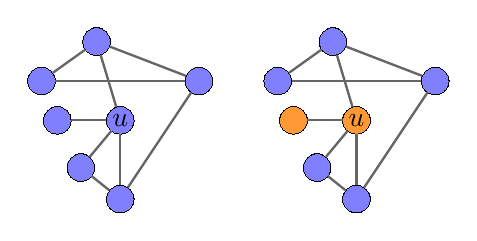
\begin{tikzpicture}[scale=1, auto,swap]

				\node[major] (v_1) at (-2, 0) {$u$};
				\node[major] (v_2) at (-2.3, 1) {};
				\node[major] (v_3) at (-2, -1) {};
				\node[major] (v_4) at (-2.8, 0) {};
				\node[major] (v_5) at (-3, .5) {};
				\node[major] (v_6) at (-2.5, -.6) {};
				\node[major] (v_7) at (-1, .5) {};

				\draw[edge] (v_1) -- (v_2);
				% \draw[edge] (v_3) -- (v_2);
				\draw[edge] (v_1) -- (v_4);
				\draw[edge] (v_7) -- (v_2);
				\draw[edge] (v_5) -- (v_7);
				\draw[edge] (v_3) -- (v_6);
				% \draw[edge] (v_3) -- (v_2);
				\draw[edge] (v_3) -- (v_1);
				% \draw[edge] (v_6) -- (v_7);
				\draw[edge] (v_1) -- (v_6);
				\draw[edge] (v_7) -- (v_3);
				\draw[edge] (v_2) -- (v_5);

				\node[minor] (u_1) at (1, 0) {$u$};
				\node[major] (u_2) at (.7, 1) {};
				\node[major] (u_3) at (1, -1) {};
				\node[minor] (u_4) at (.2, 0) {};
				\node[major] (u_5) at (0, .5) {};
				\node[major] (u_6) at (.5, -.6) {};
				\node[major] (u_7) at (2, .5) {};

				\draw[edge] (u_1) -- (u_2);
				% \draw[edge] (u_3) -- (u_2);
				\draw[edge] (u_1) -- (u_4);
				\draw[edge] (u_7) -- (u_2);
				\draw[edge] (u_5) -- (u_7);
				\draw[edge] (u_3) -- (u_6);
				% \draw[edge] (u_3) -- (u_2);
				\draw[edge] (u_3) -- (u_1);
				% \draw[edge] (u_6) -- (u_7);
				\draw[edge] (u_1) -- (u_6);
				\draw[edge] (u_7) -- (u_3);
				\draw[edge] (u_2) -- (u_5);
			\end{tikzpicture}
			\caption{Emergence of a local minority. 
			On the left hand side, a sample component from a fully-fragmented network, in which all nodes have opinion $0$ (blue). 
			On the right, the same component after a mutation and voting step, generating two opinion $1$ (orange) nodes.} \label{fig:majorities}
		\end{figure}
	
    	We now develop a closed approximation scheme by expanding around the subcritical regime. 
    	Let $\x(t) = \E[\X(t)]$. 
    	Conditioning on event types, the dynamics in $\x$ may be written
    	\begin{align}
    		m(\x(t+1) - \x(t)) = \lambda \mathbf{w}(\mathcal{G}(t)) + (1-\lambda)\alpha \mathbf{r}(\mathcal{G}(t)) + (1-\lambda)(1-\alpha) \mathbf{v}(\mathcal{G}(t))\;, \label{eq:dynamics}
    	\end{align}
    	where $\mathbf{w}$, $\mathbf{r}$, and $\mathbf{v}$ are functions of the graph state $\mathcal{G}(t)$ giving the increments in $\x$ due to mutation, rewiring, and voting, respectively. 
    	Importantly, $\mathbf{w}$ and $\mathbf{r}$ depend only on $\q$ and $\x$, the first and second moments of $\mathcal{L}$. 
    	The mutation term may be written 
    	\begin{align*}
    		w_{ij}(\mathcal{G}) = w_{ij}(\x) = 
    		\begin{cases}
    			c(x_{10} - x_{00}) &  i = j = 0 \\ 
    			c (x_{01}-x_{11}) & i = j = 1 \\ 
    			c (x_{00}  - x_{10}+x_{11}-x_{01}) & i \neq j\;.
    		\end{cases}
    	\end{align*}
    	To compute the rewiring term $r$, we write 
    	\begin{align*}
    		\mathbf{r}(\mathcal{G}) = \mathbf{r}=(r_{00}, r_{01}, r_{10}, r_{11}) = 
    		\begin{cases}
    			\left(\q_0, -\frac{1}{2}, -\frac{1}{2}, \q_1\right) & \text{rewire-to-random}\\
    			\left(1, -1, -1, 1\right) & \text{rewire-to-same}.
    		\end{cases}
    	\end{align*}
    	Unfortunately, the voting function $\mathbf{v}$ cannot be similarly parsed in any fixed, finite set of system moments.  
    	We may therefore view the short-timescale dynamics of $\x$ for fixed $\q$ as the superposition of Markovian opinion-switching and rewiring processes with a non-Markovian voting process. 
	
		Our analytical strategy is to replace the non-Markovian voting term with a Markovian approximation near the phase transition using the asymmetry between local minorities and majorities. 
		That is, we will suppose that 
		\begin{align}
			\mathbf{v}(\mathcal{G}) \approx \hat{\mathbf{v}}(\q, \x)\;, \label{eq:markov}
		\end{align}
		when $\rho \ll \frac{1}{2}$. 
		This assumption closes \Cref{eq:dynamics} in $\x$, and therefore constitutes a first-order Markovian assumption on $\x$ as a function of $\q$. 
		We fix node $u$, and suppose that at some initial time $u$ changed its opinion from $j \in \{0,1\}$ to $i \in \{1,0\}$ through either random opinion-switching or a voting step. 
		As a result of this event, $u$ now possesses a  random number $J_0$ of inactive and a random number $K_0$ of active edges. 
		The distributions of $J_0$ and $K_0$ depend on $\q$, $\x$, $c$, and potentially higher-order moments as well. 
		To compute $\hat{\mathbf{v}}$, we track each of the $K_0$ active edges until each of them has been made inactive, logging voting events along the way.
		Approximating the impact of these events on the active edge count and averaging thus provides our approximation $\hat{\mathbf{v}}$ for $\mathbf{v}$.
		
		Under timescale separation and mean-field   assumptions, these calculations may be carried out in closed form. 
		The timescale separation assumption supposes that $\mathcal{G}$ is changing slowly relative to the ego network of node $u$, so that only update steps that sample the initial $K_0$ edges require accounting. 
		This assumption will be strongest when the active edge density $\rho$ and mutation rate $\lambda$ are both small. 
		The mean-field assumption supposes that nodes in the local majority have degree distributions governed by the global network average $\x$. 
		This assumption reflects the fact that, for small $\rho$, most nodes are by definition members of their respective local majorities. 
		This allows us to approximate the distributions of $J_0$ and $K_0$ in terms of $\q$ and $\x$. 
		It is useful to define the vector $\C$ with components $c_{ij} = c{x_{ij}}/{q_i}$ denoting the average number of neighbors of type $j$ of a node of type $i$. 
		Note that, while $x_{ij} = x_{ji}$, $c_{ij} \neq c_{ji}$ for $\q \neq \left(\frac{1}{2}, \frac{1}{2}\right)$.
		Under the mean-field assumption, $\E[K_0] = c_{00}$. 
		Meanwhile, $\E[J_0] = 1 + c_{01}$ if $u$ emerged as a forward vote, and $\E[J_0] = 0$ if $u$ emerged as a mutation. 
		In the approximations below, we model each of $K_0$ and $J_0$ as truncated Poisson random variables with the appropriate intensities. 

		There are multiple types of voting events we need to track, and we define random variables for each. 
		\begin{itemize}
			\item \textbf{Type 1}: Neighbors of $u$ may vote. By the separation of timescales assumption, each such vote happens along one of the $K_0$ initial active edges. By the mean-field assumption, votes on these nodes are governed by the global statistics $\C$. Let $E$ denote the (random) number of such votes. 
			\item \textbf{Type 2}: $u$ itself may vote prior to all $K_0$ active edges becoming inactive. Let $G$ denote the indicator random variable for this event. 
			\item \textbf{Type 3}: Nodes not attached to $u$ may vote. In the rewire-to-random model, such voting events occur when an active edge attached to $u$ is rewired in such a way that it is no longer attached to $u$, but remains active. In the rewire-to-same model, such events do not occur. Let $F$ denote the (random) number of these events. 
		\end{itemize}

		These variables will count the voting events, but we also require vectors to track the impact of a given event on $\x$. 
		The impact on the edge count vector $\mathbf{m}$ due to Type 1 events when $\mathcal{L}_u = 1$ on a component dominated by $0$s is given by 
		\begin{align}
			\mathbf{e}_1(\C) = \frac{1}{2}\left(-2c_{00} , c_{00} - c_{01} - 1, c_{00} - c_{01} - 1, 2(1+c_{01})\right)^T\;.
		\end{align}
		Interchanging the opinion indices gives the analogous expression for $\mathbf{e}_0$, the impact of forward votes when $u$ has opinion $0$ on a component dominated by $1$s. 
		Type 3 events counted by $F$ are again mean-field approximated. 
		Since these edges are no longer connected to $u$, their impact is independent of $i$. 
		We then have
		\begin{align}
			\mathbf{f}(\C) = \frac{\mathbf{e}_0(\C) + \mathbf{e}_1(\C)}{2}\;.
		\end{align}

		It remains to consider the impact of Type 2 events, for which the analysis is more subtle. 
		This term has components
		\begin{align}
			\mathbf{g}_1(\q, \C) = \frac{1}{2}\left(2\E[K|1], \E[J-K|1], \E[J-K|1], -2\E[J|1]\right)\;, \label{eq:g_components}
		\end{align}
		where $J$ (respectively, $K$) are the number of inactive (active) edges attached to $u$ at the time of voting. 
		The expectations are again conditioned on $\mathcal{L}_u = 1$.  
		To complete the approximation scheme, it is necessary only to compute the various expectations appearing in \Cref{eq:g_components}.
        We begin with $K$, the active edge count at the time that $u$ votes. 
        Conditioned on a fixed initial number $k_0$ of active edges, $K$ is distributed as a truncated geometric distribution: 
        \begin{align*}
        p_{K|I, K_0}(k|i, k_0) = 
        \begin{cases}
          (1-\beta_i)\beta_i^{k_0 - k} &\quad 1\leq k \leq k_0\\ 
          \beta_i^{k_0} &\quad k = 0,
        \end{cases}
        \end{align*}
        where $\beta_i$ is the probability that an event is not a vote by $u$, given that it removes a discordant edge from $u$. 
        This probability is given analytically by 
        \begin{align}
        \beta_i \triangleq 
        \begin{cases}
          \frac{1+\alpha q_i}{2-\alpha(1-q_i)} &\quad \text{rewire to same}\\ 
          \frac{1+\alpha}{2} &\quad \text{rewire to random.} \label{eq:beta}
        \end{cases}
        \end{align}
        We may now begin to compute expectations.
        First, the probability of $u$ voting prior to deactivation, conditioned on $K_0$, is  
        \begin{align*}
        \E[G|K_0, i]  &= \prob(K \geq 1) \\ 
                 &= 1-\beta_i^{K_0},
        \end{align*}
        Averaging over $K_0$ yields 
        \begin{align*}
        \E[G|i] = \sum_{k_0}p_{K_0}(k_0)(1-\beta_i^{k_0}) = 1 - \phi_{K_0}(\beta_i)\;,
        \end{align*}
        where $\phi_{K_0}(z) = \sum_{k = 1}^\infty \prob(K_0 = k) z^{k}$ is the probability generating function of $K_0$. 
        Next, the expected number of active edges given that $u$ votes is 
        \begin{align*}
        \E[GK|i] &= \E_{K_0}\E[GK|i, K_0] \\ 
                    &= \E_{K_0}\left[K_0 - \frac{\beta_i(1-\beta_i^{K_0})}{1-\beta_i}|i\right] \\ 
                    &= \E[K_0|i] - \frac{\beta_i}{1-\beta_i}(1-\phi_{K_0}(\beta_i))\;.
        \end{align*}
        
        To compute the remaining terms, it is useful to define the coefficients 
        \begin{align*}
        \eta_i \triangleq 
        \begin{cases}
          \frac{1-\alpha(1-q_i)}{1+\alpha q_i}\,,  \\ 
          \frac{1-\alpha}{1+\alpha}\,,
        \end{cases} \quad 
        \rho_i \triangleq 
        \begin{cases}
          \frac{1-\alpha}{1+\alpha q_i}\,,  \\ 
          \frac{1-\alpha}{1+\alpha}\,,   
        \end{cases} \quad 
        \sigma_i \triangleq 
        \begin{cases}
          \frac{2(1-\alpha)}{2-\alpha}\,, &\quad \text{rewire to random}\,, \\ 
          0\,,   &\quad \text{rewire to same.}
        \end{cases} \label{eq:coefs}
        \end{align*}
        The coefficient $\eta$ gives the probability that an event that removes an active edge from $u$, other than a vote by $v$, produces an inactive edge either through rewiring or through a vote by a neighbor of $v$. The coefficient $\rho$ gives the probability that such an event is in fact a vote by a neighbor of $v$. The coefficient $\sigma$ gives the probability that an active edge which is rewired but not resolved is ultimately resolved via a vote. 
        
        Node $u$ gains inactive edges via rewiring and voting at rate $\eta_i$. 
        The expected number of inactive edges at the time of that $u$ votes is therefore 
        \begin{align*}
        \E[GJ|i] &= \E_{K_0}\left[\E[J_0|i, K_0] + \eta_i \left(\E[K_0|i] - \E[GK|i, K_0]\right)\right] \\
                    &= \E[K_0|i] + \eta_i \left(\E[K_0|i] - \E[GK|i]\right)\;.
        \end{align*}
        Next, the expected number $\E[E|i]$ of Type 1 events  can be calculated simply by noting that a voting event along edge $(u,v)$ has equal probability to change $\mathcal{L}_u$ as $\mathcal{L}_v$. 
        As a result, the expected number of Type 1 events is equal to the expected number of votes by $u$ itself, which is simply $\E[G|i]$. We thus obtain 
        \begin{align*}
        \E[E|i] = \E[G|i] = 1 - \phi_{K_0}(\beta_i)\;. 
        \end{align*}
        Next, we consider Type 3 events prior to a vote by $u$. 
        For a Type 3 event to occur, the voting edge must be no longer attached to $u$. 
        The expected number of such edges is $\E[K_0 + J_0 - G(K - J)|i]$. 
        The probability that such an edge was removed by $u$ by a rewiring event that did not resolve the edge is $\sigma_i$. 
        We thus have 
        \begin{align*}
            \E[W|i] = \sigma_i\E[K_0 + J_0 - G(K - J)|i]\;.
        \end{align*}
        
        Note that, although Type 1 and Type 2 events occur at the same rate, their expected impacts on the vector of edge counts are different. 
        Since $\E[K|i] < \E[K_0|i]$ and $\E[J|i] > \E[J_0|i]$, we have   
        \begin{align}
            \mathbf{e}_i(c)_{01} = \frac{\E[K_0|i] - \E[J_0|i]}{2} > \frac{\E[K|i] - \E[J|i]}{2} =   
            -{g}_i(q,c)_{01}\;.
        \end{align}
        That is, a Type 1 event increases the active edge density more than a Type 2 event decreases it. 
        This reflects a form of local symmetry-breaking in votes favoring local minority and local majority opinions. 
        Intuitively, the broken symmetry is due to the intervening rewiring-steps, which remove edges from $u$ prior to a Type 3 event, but which do not operate on nodes which vote in a Type 1 event due to the separation of timescales assumption. 
        Since Type 1 and 2 events happen at the same rate, this formalism gives concrete quantitative insight into why voting events tend to increase the active edge-density for small $\rho$. 
        
        
        
        

		\begin{figure}
			\centering
				\includegraphics[width=1\textwidth]{transition_joy}
			\caption{Approximating the phase transition. 
			Grey ridges give simulation traces of $\rho$ from networks with $n = 10^4$ nodes, $\lambda = 2^{-16}$, and varying $c$ and $\alpha$. 
			The green curve gives the prediction of the phase transition found by numerically solving \Cref{eq:transition_approx} via least-squares. 
			The orange curve gives the pair approximation (PA) as derived in \cite{Durrett2012} for each model variant.}
			\label{fig:transition_joy}
		\end{figure}
        
        Finally, we may average over Type 1, 2, and 3 events to obtain the expected increment in edge counts per voting event. 
        It is given by the 4-vector 
		\begin{align}
			\hat{\mathbf{v}}(\q, \x) = \frac{1}{2} \sum_{i \in \{0,1\}} \frac{\E[E|i]\mathbf{e}_i(\C) + \E[F|i]\mathbf{f}(\C) + \E[G\mathbf{g}_i(\mathbf{q},\mathbf{c})|i]}{\E[E + F + G|i]}\;. \label{eq:v_hat}
		\end{align}
		With \Cref{eq:v_hat} in place, we may then approximate the long-term dynamics of $\x$ under \Cref{eq:dynamics}. 
		We write $\hat{\x}(\q; \alpha)$ for the limit point of the dynamics. \todo{Uniqueness of $\hat{\x}$?}
		The approximation is subcritical when $\hat{\rho}(\q; \alpha) \triangleq 2\hat{\x}_{01}(\q; \alpha) = 0$, and supercritical otherwise. 
		Solving 
		\begin{align}
			\alpha^*(\q) = \max \{\alpha : \hat{\rho}(\q; \alpha) = 0\} \label{eq:transition_approx}
		\end{align}
		gives our approximation for the phase transition. 

		\Cref{fig:transition_joy} shows the approximate phase transitions computed using \Cref{eq:transition_approx} for varying $c$, in green, when $\q = \left(\frac{1}{2}, \frac{1}{2}\right)$. % \footnote{Empirically, the rewire-to-random curve phase transition can also be computed by solving $\phi_{K_0}(\beta_i^{K_0}) \approx \frac{1}{2}$ for $\alpha$, which has a branching-process intuition behind it and leads to a much cleaner calculation. Intriguingly, the right constant for the rewire-to-same case appears to be $\phi_{K_0}(\beta_i^{K_0}) \approx \frac{1}{3}$} 
		Compared to the standard pair approximation (orange), the present approximation approach is substantially more accurate.
		Indeed, the calculation of the transition for the rewire-to-random model is the most accurate we know of, while the calculation for the rewire-to-same model is competitive with existing approaches.
		The approximation of the phase transition is more accurate than the Approximate Master Equations (AMEs) of \cite{Durrett2012} and the partial differential equation approach of \cite{Silk2014}. 
		The fan-motif method used by \cite{Bohme2011} to estimate the rewire-to-same phase transition is somewhat more accurate in that case, but also much higher-dimensional, requiring a bisection search in $\alpha$ in which each stage computes the leading eigenvalue of a $(c-1)\times (c-1)$ matrix. 

		As discussed in \cite{Durrett2012} and shown in \Cref{fig:arch_illustration}, the phase transitions in the two models differ in their sensitivity to $\q$. 
		This behavior is reflected algebraically in \Cref{eq:beta,eq:coefs}, which define the coefficients appearing in \Cref{eq:v_hat}. 
		These coefficients depend directly on $\q$ in the rewire-to-random case, regardless of the value of $\x$. 
		However,  in the rewire-to-same model, dependence on $\q$ emerges only when $\rho > 0$, implying that the phase transition itself is independent of $\q$. 
		Furthermore, the local approximation scheme also gives us a direct interpretation of this mysterious behavior. 
		Consider the emergence of a mutant node $u$ with opinion $1$ on a component of majority opinion $0$. 
		In the rewire-to-random case, the fast local rewiring dynamics depend explicitly on $\q$, the \emph{global} opinion densities. 
		When $\q_1$ is large, an edge attached to $u$ and rewired is more likely to become inactive, resulting in fewer active edges in the neighborhood of $u$. 
		In the rewire-to-same case, however, the fast rewiring does not explicitly depend on $\q$. 
		An active edge attached to $u$ and rewired becomes inactive with probability $1$, regardless of the value of $\q$. 
		The local dynamics are not fully independent of $\q$, but the dependence is mediated by the slow voting dynamics. 
		% \pjm{This intuition is really good here. I'm curious, there also seems to be a way in which the model for rewire-to-same has a degenerate behavior at small $\rho$ in that it also implies that one of the opinions is of small population, so then three of the edge types are small. I'm just babbling...}\pc{I'm interested in where you're going here. At the moment, I can't see the distinction between the two models along these lines -- want to elaborate?}\pjm{It's very possible it wasn't a well-formed thought on my part (smile). I think I was trying to observe that in principle the only time the $\rho$ near zero for rewire-to-same should be stable is if one of the 2 opinions was all but vanished. But this might not be useful for anything. Feel free to comment this discussion away.}
	
		We now turn to the approximation of $\rho^*(\q;\alpha)$, the equilibrium density of active edges, for $\alpha < \alpha^*$. 
		In this regime, the distinction between local minority and majority nodes progressively erodes, along with the separation of timescales assumption. 
		One way to view this erosion is in terms of backward votes: the impact of a single node voting backwards progressively diminishes due to re-randomization of the node's local neighborhood between votes. 
		We model this re-randomization via simple interpolation to an approximation of the case $\alpha = 0$, which corresponds to a variation of a ``pure'' voter model without rewiring. 
		A simple mean-field argument (given in \Cref{sec:SI_alpha_0}) provides an approximation for the $\alpha = 0$ arch:
		\begin{align}
			\hat{\rho}^*(\q; 0) \approx 2q_0q_1\frac{c-1}{c}\;. \label{eq:alpha_0}
		\end{align}
		We note in passing that, despite the crudeness of this mean-field approximation, this estimate is substantially more accurate than both the pair approximation in \cite{Durrett2012} and the even more sophisticated active-motif approach of \cite{Demirel2012}. 

		We introduce the interpolation function 
		\begin{align}
			s(\x) = \frac{\hat{\rho}^*(\q;0) - \rho}{\hat{\rho}^*(\q;0)}\;, \label{eq:interpolation}
		\end{align}
		to quantify the distance of the system state from the estimated $\alpha = 0$ arch, and then use this interpolation function to introduce decay in the backward voting term  \Cref{eq:g_components},\footnote{While any monotonic transformation of  \Cref{eq:interpolation} may be well-motivated, in practice we found similar numerical results under a variety of such transformations.}
		replacing $\mathbf{g}(\q, \C)$ in \Cref{eq:v_hat} with $\tilde{\mathbf{g}} = \mathbf{g}(\q, \C)s(\x)$.
		The corresponding solution for $\x$ then yields our approximation of $\mathbf{\rho}$. 
		\begin{figure}
			\centering
				\includegraphics[width=.8\textwidth]{arch_tops}
			\caption{Supercritical equilibria for $\q = \left(\frac{1}{2}, \frac{1}{2}\right)$.
			Dots give simulation traces from a network of $n = 10^4$, $\lambda = 2^{-12}$, and varying $\alpha$ and $c$.
			Solid lines give the approximation to $\rho$ computed by numerically solving \Cref{eq:dynamics} using \Cref{eq:v_hat} and the supercritical interpolation \Cref{eq:interpolation}.} \label{fig:arch_tops}
		\end{figure}
		
		To evaluate the supercritical approximation, we first consider its performance on the common estimation task with $\q = \left(\frac{1}{2}, \frac{1}{2}\right)$. 
		\Cref{fig:arch_tops} shows the estimate for $\rho$ when $\q = \left(\frac{1}{2}, \frac{1}{2}\right)$ for varying $\alpha$. 
		The rewire-to-random approximation is strikingly accurate. 
		Even the worst-case approximation ($c = 4$) deviates from simulations by no more than $5\%$.
		This  level of accuracy is comparable with that of the  Approximate Master Equation (AME) approach employed in \cite{Durrett2012}. %\pjm{Is it really? Isn't it actually better than the AME result in the Durrett et al. paper? Or are you just being conservative? (Not that there's anything wrong with that!)}\pc{Checking Fig. 10 of \cite{Durrett2012}, it looks like the largest deviation from the data occurs with $\alpha = 0.7$, with a discrepancy $\hat{\rho} - \rho \approx 0.07$ or so, when $c = 4$. The largest deviation for $c = 4$ in our model is around $\alpha = 0.6$ or so, and is maybe $\hat{\rho} - \rho \approx 0.05$ -- better, not wildly. Of course we have advantages -- better near the phase transition, and we can compute for larger $c$. But if you made a version of this plot with AMEs, at least for $c = 4$, it would look a bit better than I think you think it would. =)}
		Furthermore, whereas AMEs become prohibitively computationally intensive for larger $c$, our approximation yields near-exact predictions. 
		Interestingly, the two methods are most accurate in dramatically different regimes---whereas the AMEs are nearly exact for small $\alpha$ and decay in quality near $\alpha^*$, our present method is much more accurate near $\alpha^*$ but degrades slightly as $\alpha$ becomes small. 
		In the rewire-to-same case, the approximation is predictably weaker due to the larger error in the estimation of the phase transition. 
		There is larger deviation, on the order of $10\%$, in many of the simulation traces depending on $c$. 
		The overall approximation quality is again comparable to that of AMEs, but is outperformed by certain specialized methods such as the active-motif approach of \cite{Demirel2012}. 
		
		Turning now to the case $\q \neq \left(\frac{1}{2}, \frac{1}{2}\right)$, \Cref{fig:arches} compares the curves obtained by numerically solving \Cref{eq:dynamics} as $\q$ varies. 
		Due to the accurate estimation of the location of the phase transition in $\alpha$, the arches for the rewire-to-random model agree well with the data both on the equilibrium active edge density and on the support of the arch---the values of $\q$ for which $\rho^*(\q;\alpha) > 0$. 
		Compared to AMEs, the computed arches for the $c = 4$ rewire-to-random case are comparable in overall accuracy, better estimate the correct support, and also better capture the qualitative parabolic shape.  
		The accuracy of the approximation increases with $c$, but comparison to AMEs and active-motif approaches are no longer possible due to the computational costs of the latter two methods. 
		As with the $\q = \left(\frac{1}{2}, \frac{1}{2}\right)$ case, the rewire-to-same results are less accurate. 
		The computed arches for the rewire-to-same case do correctly span the entire interval $[0,1]$ and 
		the overall numerical accuracy in the $c = 4$ case is comparable to AMEs, but the qualitative parabolic shape has suffered a significant amount of warping near its base. 
		The reason for this difference is not clear to us and we note further investigation into this phenomenon may be called for. 

		\begin{figure}
			\centering
				\includegraphics[width=1\textwidth]{arches}
			\caption{Approximations to arches for rewire-to-random and rewire-to-same systems with varying mean degree $c$ and rewiring rate $\alpha$. 
			Curves give theoretical predictions obtained by numerically solving \Cref{eq:dynamics} using \Cref{eq:v_hat} and the supercritical interpolation \Cref{eq:interpolation}. 
			Points give simulation averages traces from networks with $n = 10^4$ nodes,  $\lambda = 2^{-16}$, and varying $\alpha$.}
			\label{fig:arches}
		\end{figure}

		In addition to demonstrating favorable accuracy, the present approximation approach is much lower-dimensional than its competitors. 
		AMEs require the solution of $\Theta\left(k_\mathrm{max}^2\right)$ coupled differential equations; in the $c = \langle k\rangle = 4$ case, the authors of \cite{Durrett2012} used $225$ such equations. 
		This makes the computation of equilibrium approximations computationally prohibitive for even moderate $c$. 
		Active-motif methods also have similar scaling properties. \todo{What actually IS the difference between active-motif methods and AMEs?}
		In contrast, the present method displays constant scaling: there are four nonlinear equations to solve, regardless of the value of $c$. 
		The low-dimensional nature of the approximation also supports useful intuition in that each term meaningfully corresponds to a distinctive event type.


\section{Discussion} \label{sec:discussion}

	Adaptive voter models offer a simple set of mechanisms that generate emergent opinion-based assortativity in complex networks. 
	While the underlying rules are simple to state, the coevolving nature of the dynamics render these systems very challenging to analyze. 
	We have considered an ergodic adaptive voter model variant which enables a local perspective on fragmentation transitions and other model properties. 
	The local perspective allows us to use the asymmetry of voting events to develop Markovian approximations based on the fast timescale dynamics around single nodes. 
	The resulting approach is conceptually intuitive, computationally tractable, and empirically accurate. 
	
	One of the most puzzling issues raised by our results is the difference between the accuracies of our approach for the rewire-to-random and rewire-to-same adaptive voter models. 
	While we succeed in characterizing the rewire-to-random arch nearly exactly, the same methods produce poorer results for the rewire-to-same model. 
	We conjecture that the rapid local sorting produced in rewire-to-same dynamics badly violates our mean-field assumption on forward votes, as suggested by the bottom-left panel of \Cref{fig:symmetry_breaking} (\Cref{sec:symmetry_breaking}, Appendix). 
	It would be interesting to extend our methodology to see whether refinements are possible that better characterize the rewire-to-same behavior, and potentially shed light on the essential features governing the dramatic difference in the nature of the phase transitions in these two models. 
		
	It is also of substantial interest to consider extensions and generalizations. 
	The most natural extension is to the case of multiple opinion states and structured opinion spaces. 
	Previous work on multi-opinion models has been restricted to either characterization of the various phase transitions \cite{Bohme2012} or empirical discussion of supercritical equilibrium behavior \cite{Shi2013}. 
	One explanation for this limitation in scope is computational, in that the number of operations required to compute approximations under active-motif and AME approaches are exponential in the number $\abs{\mathcal{X}}$ of opinion states, rendering both methods infeasible. 
	In contrast, likely extensions of our moment-closure methods scale as $\Theta(\abs{\mathcal{X}}^2)$, which could be computationally tractable. 
	If accuracy were preserved, such extensions would present the first scalable analytic methods for multi-opinion models. 
	%Further generalizations may also be possible. 
	While we developed our approximations for the specific case of the binary-state AVM, that development relies only on ergodicity, timescale separation, and the mean-field assumption. 
	We conjecture that these ingredients should be present in any adaptive model with homophilic dynamics in which rewiring steps involve uniform selection from an extensive subset of the graph, such as a subset sharing a given node state. 
	An example of a more complex system in which these ingredients are present is the networked evolutionary prisoner's dilemma game of \cite{Lee2018}, in which nodes display richer strategic behavior in their opinion update and rewiring behavior. 
	Despite this, the existence of a phase transition driven by homophily may allow for the deployment of our novel methods in such cases as well. 
	% An example coevolutionary model to which our methods may not be applicable is the transitivity-reinforced dynamics of \cite{Malik2016}. 
	% Because nodes tend to rewire within their neighborhoods, timescale separation may not be a practical assumption. 

	
\section*{Acknowledgments} 
	We are grateful to Feng (Bill) Shi for contributing code used for simulations, and to Patrick Jaillet for helpful discussions. PSC was supported by an NSF Graduate Research Fellowship under Grant Number 1122374. PJM was supported by the Eunice Kennedy Shriver National Institute of Child Health \& Human Development of the National Institutes of Health under Award Number R01HD075712. The content is solely the responsibility of the authors and does not necessarily represent the official views of the National Science Foundation or National Institutes of Health. %\pc{Amused by the thought that our views here could get NIH in trouble if we didn't have that disclaimer.} HA!

% TODO
%%% Reverse-outline, with special emphasis on introduction, discussion, conclusion.
%%% Revise appropriately
%%% Standardize notation, and consolidate SI
%%% Check figures

\bibliographystyle{siamplain}
\bibliography{refs.bib}{}

\section{Appendix}

    \subsection{Symmetry-Breaking in Simulation Traces} \label{sec:symmetry_breaking}
        In \Cref{sec:analytic}, we noted that the algebra of our approximation predicts an asymmetry between votes in favor and against the local minority.
        In particular, votes in favor of the local minority increase the active edge density more than votes against decrease it. 
        This asymmetry can be qualitatively observed in simulation data, shown in \Cref{fig:symmetry_breaking}. 
        \begin{figure}
			\centering
				\includegraphics[width=1\textwidth]{symmetry_breaking}
			\caption{Histograms giving the increase in active edge density per voting event for rewire-to-random and rewire-to-same AVMs with $n = 10^4$ nodes, $c = 8$, and $\lambda = 2^{-16}$. The black vertical gives the mean of the distribution. The red vertical gives the explicit approximation $2e_i(c)_{01}$ for the impact due to forward votes when $\rho = 0$.}
			\label{fig:symmetry_breaking}
		\end{figure}
		The asymmetry between events is manifest in the skewed, bimodal distribution of voting impacts for small $\rho$. 
		As $\rho$ increases, the distinction between local minorities and majorities erodes, gradually resulting in a symmetric, unimodal distribution. 
        
    \subsection{Mean-Field Approximation for $\alpha = 0$} \label{sec:SI_alpha_0}
        In this section, we derive \Cref{eq:alpha_0} of the main text, which gives a mean-field approximation for the arch in the case $\alpha = 0$. 
        In this case, active edges enter and exit the system only via voting events. 
        The mean-field approximation for the impact of a voting event is $g(\C) = \frac{1}{2}\left(g_0(\C) + g_1(\C)\right)$, where $g_i(\C)$ is defined in \Cref{eq:g_components}. 
        The equilibrium condition is $g(\C) = 0$. 
        Since $\C$ lives in a 2-dimensional subspace of $\R^4$, it suffices to solve the system
        \begin{align*}
        	0 &=  1 + c_{10} - c_{00} \\ 
        	0 &=  1 + c_{01} - c_{11} 
        \end{align*}
        for $\C$ and subsequently for $\x$.  
        We recall that $c_{ij} = c{x_{ij}}/{q_i}$ and that $2x_{01} = 1 - x_{00} - x_{11}$. 
        Substituting these relations we obtain
        \begin{align*}
        \frac{2q_0q_1}{c}\mathbf{1} + \q = \left[\begin{matrix} 1 + q_1 & q_0 \\ q_1 & 1 + q_0 \end{matrix}\right]\left(\begin{matrix}x_{00} \\ x_{11}\end{matrix}\right)\;.
        \end{align*}
        The unique solution is 
        \begin{align*}
        \left(\begin{matrix}x^*_{00} \\ x^*_{11}\end{matrix}\right) = \frac{q_0 q_1}{c} \mathbf{e} + \frac{1}{2}\left(\begin{matrix} q_0(1 + q_0 - q_1) \\ q_1(1 + q_1 - q_0) \end{matrix}\right)\;.
        \end{align*}
        We may then compute the arch: 
        \begin{align*}
        \rho^*(\q) = 2x_{01} 
             = 1 - x^*_{00} - x^*_{11} 
             = 2q_0 q_1 \frac{c-1}{c},
        \end{align*}
        as was to be shown. 

\end{document}